
\section{Preliminaries}
In this section, we first give an overview of our whole work. And we will introduce the notations used in this paper and problem definitions in our task.

\subsection{Overview}
\begin{figure}[htb]
    \centering
    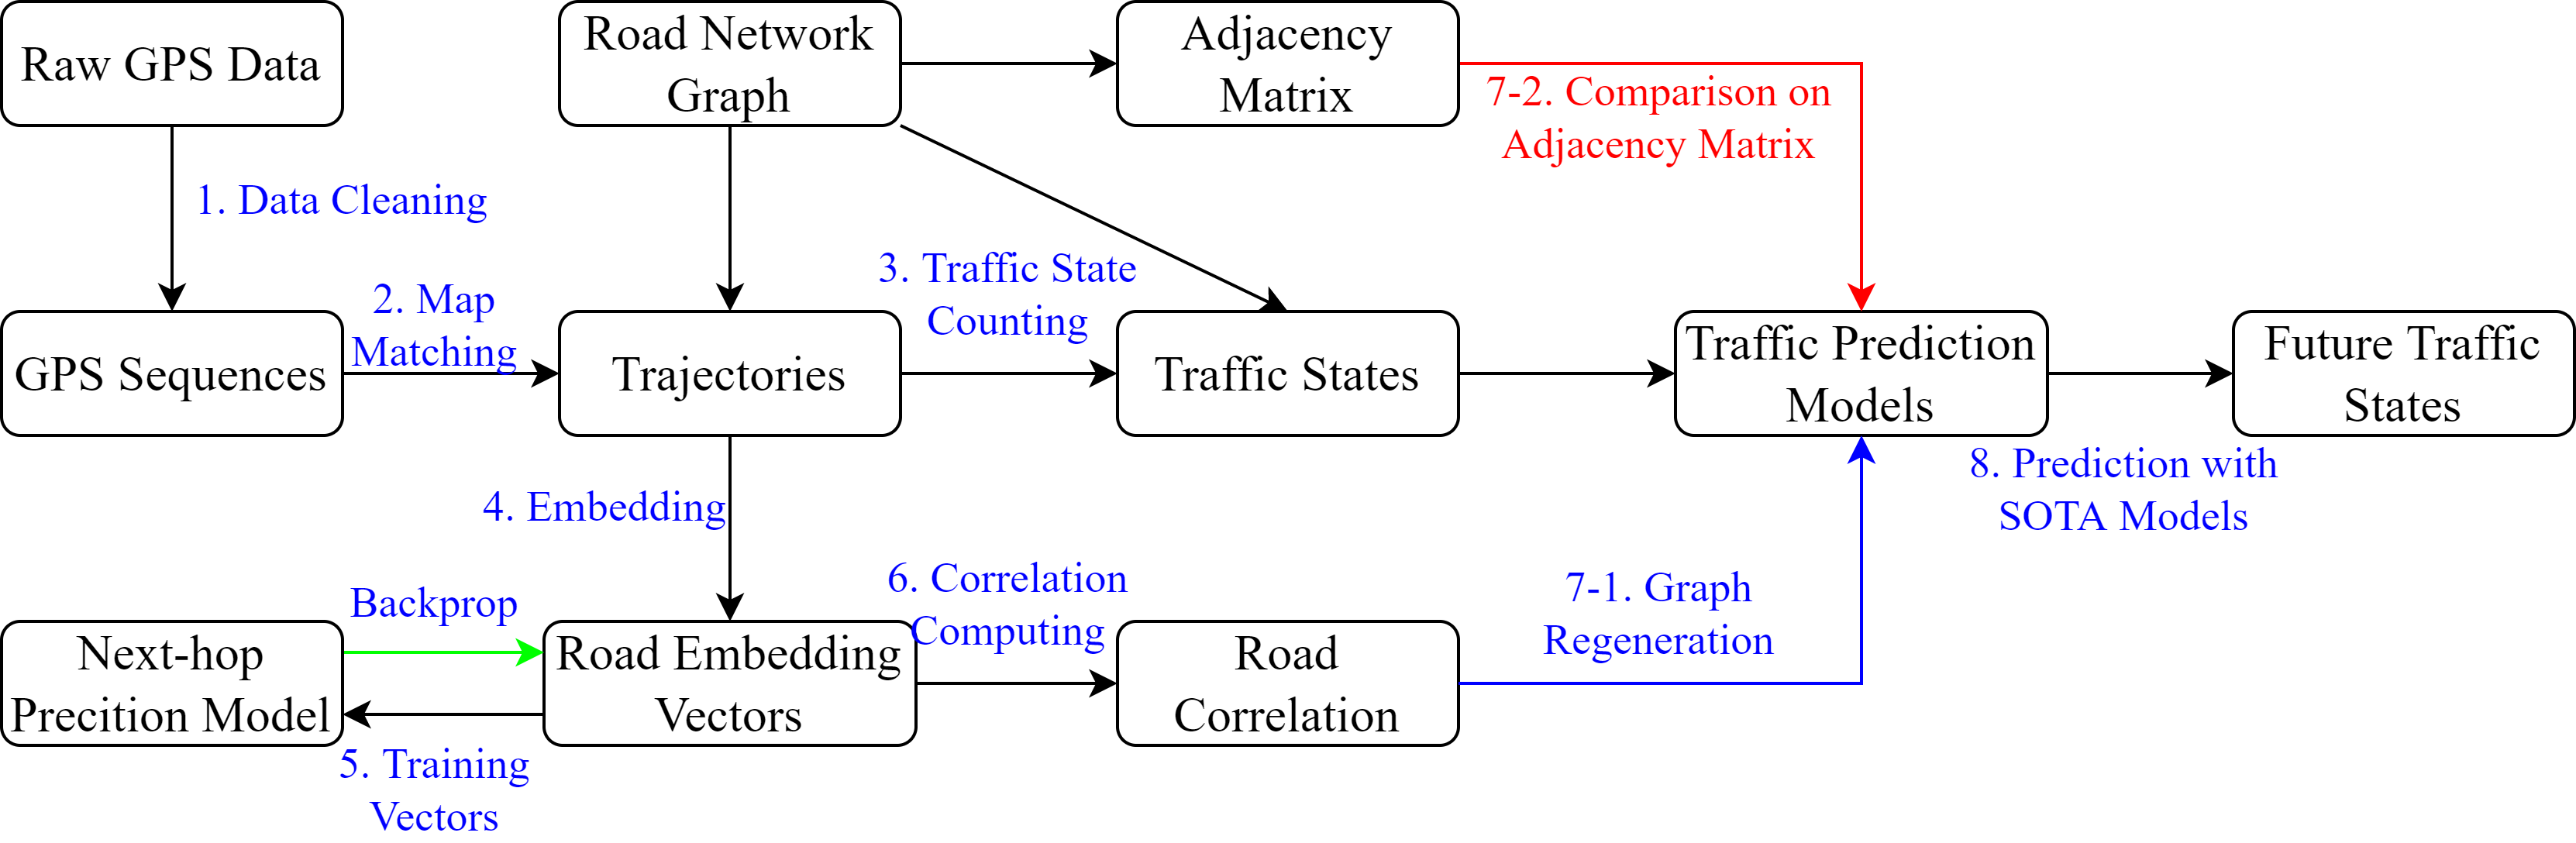
\includegraphics[width=\textwidth]{images/overview.drawio.png}
    \caption{An overview of our work.}
    \label{fig: overview}
\end{figure}

Figure \ref{fig: overview} provides an overview of this paper, and the details of each part will be stated in the following sections. Section 4 introduces how we build the dataset. The adopted methodology and model structure will be given in section 5. In section 6, the proposed model is verified by our dataset, and the experiment results demonstrate its practicability. A brief conclusion and several potential directions are provided in the last section.

\subsection{Notations}
Table \ref{notation_table} gives the notations and their definitions.
\begin{table}[h!]
    \begin{center}
        \caption{Notations}
        \label{notation_table}
        \begin{tabular}{cl}
            \toprule

            \textbf{Notation} & \textbf{Definition}                       \\

            \midrule

            $n_{(\cdot)}$     & number of some entities                   \\
            $d_{(\cdot)}$     & vector dimension                          \\
            $\mathcal R$      & road set                                  \\
            $r$               & a single road in $\mathcal R$             \\
            $\mathcal E$      & edge set                                  \\
            $A$               & adjacency matrix                          \\
            $\mathcal G$      & road network graph                        \\
            $\mathcal T$      & trajectory set                            \\
            $T$               & a trajectory in $\mathcal T$              \\
            $ts$              & timestamp                                 \\
            $s$               & speed                                     \\
            $w$               & window size                               \\
            $p$               & random sampling proportion                \\
            $E$               & road embedding matrix                     \\
            $\mathbf{e}_i$    & embedding vector for road $r_i$           \\
            $C$               & road correlation matrix                   \\
            $t$               & time interval                             \\
            $X$               & traffic state matrix                      \\
            $\mathbf x_t$     & traffic state vector at time interval $t$ \\

            \bottomrule
        \end{tabular}
    \end{center}
\end{table}

\subsection{Problem Definition}
This subsection gives the definitions\cite{AAAI21} of the concepts and tasks occur in this paper.
\begin{definition}[Road Network Graph]
    The road network can be represented by a directed graph $\mathcal{G}=(\mathcal{R}, \mathcal{E}, A)$, where $\mathcal{R}=\{r_1, r_2, \dots, r_{n_r}\}$ is a finite set of roads that each $r_i$ stands for a real road in the road network, which is an integer ID in practice. $\mathcal{E}$ is the set of directed edges where $(r_i, r_j)\in \mathcal{E}$ indicates that there is a directed edge from $r_i$ to $r_j$, i.e. $r_j$ is the downstream road in the road network. $A \in [0, 1]^{n_r\times n_r}$ is the adjacency matrix whose entry $A_{i, j}$ is a binary value that indicates whether there exists an edge $(r_i, r_j)\in\mathcal{E}$.
\end{definition}

\begin{definition}[Trajectory]
    Given a road network graph $\mathcal{G}=(\mathcal{R}, \mathcal{E}, A)$, a trajectory $T=[(r_1, s_1, ts_1), (r_2, s_2, ts_2), \dots, (r_l, s_l, ts_l)]$ is a sequence of (road, speed, timestamp) tuples. Each tuple $(r_i, s_i, ts_i)$ specifies that the vehicle is driving on $r_i$ with speed $s_i$ at timestamp $ts_i$. Besides, $\forall i=1, 2, \dots, l-1$, $r_i\neq r_{i+1}$ and $(r_i, r_{i+1})\in\mathcal{E}$.
\end{definition}

\begin{definition}[Traffic State]
    Traffic state stands for the traffic flow or speed of a road during a particular time interval. Traffic flow is defined as the number of vehicles passing by the road, and traffic speed is the average speed of these vehicles. For a road graph $\mathcal{G}=(\mathcal{R}, \mathcal{E}, A)$, we use $X\in\RR^{n_r\times n_t}$ to record the traffic state of each time interval. For time interval $t$, $\mathbf{x}_t=X_{:, t}\in\RR^{n_r}$ represents the traffic state of all roads during $t$.
\end{definition}

\begin{problem}[Next-hop Prediction]
    Given a road network graph $\mathcal{G}=(\mathcal{R}, \mathcal{E}, A)$ and the road sequence in a trajectory $T^r=\{r_1, r_2, \dots, r_l \}$ with length $l$, the trajectory next-hop prediction is to obtain a probability distribution $\hat P$ on road set $\mathcal{R}$ that best predicts the next step $r_{l+1}$. In conclusion, our goal is to build a model with parameters $\Theta$ that satisfies
    \begin{equation}
        \Theta=\mathop{\arg\min}_\Theta CrossEntropy(\hat P, P)
    \end{equation}
\end{problem}

\begin{problem}[Road Correlation]
    Given a road network graph $\mathcal{G}=(\mathcal{R}, \mathcal{E}, A)$, find a road correlation function $Cor$ which takes two roads as input and returns a real number $Cor(r_i, r_j)$ to quantify the spatial dependency between two roads $r_i$ and $r_j$. The value is bigger if the two roads have a stronger dependency. The road correlation matrix $C\in\RR^{n_r\times n_r}$ stores all the correlation values s.t. $C_{i, j}=Cor(r_i, r_j)$.
\end{problem}

\begin{problem}[Traffic State Prediction]
    Given a road network graph $\mathcal{G}=(\mathcal{R}, \mathcal{E}, A)$, find a function $f$ and its parameter set $\Theta$ s.t. given historical traffic states $\{\mathbf{x}_{t-w_{in}+1}, \mathbf{x}_{t-w_{in}}, \dots, \mathbf{x}_t \}$ for an input window $w_{in}$, $f$ estimates the most likely traffic states $\{\mathbf{x}_{t+1}, \mathbf{x}_{t+2}, \dots, \mathbf{x}_{t+w_{out}} \}$ for an output window $w_{out}$.
    \begin{equation}
        \begin{aligned}
            \hat X_{:, t+1:t+w_{out}}&=f_\Theta(X_{:, t-w_{in}+1:t-1})\\&=\mathop{\arg\max}_{X_{:, t+1:t+w_{out}}} p(X_{:, t+1:t+w_{out}}|X_{:, t-w_{in}+1:t-1})
        \end{aligned}
    \end{equation}
\end{problem}
